%%%%%%%%%%%%%%%%%%%%%%% file template.tex %%%%%%%%%%%%%%%%%%%%%%%%%
%
% This is a general template file for the LaTeX package SVJour3
% for Springer journals.          Springer Heidelberg 2010/09/16
%
% Copy it to a new file with a new name and use it as the basis
% for your article. Delete % signs as needed.
%
% This template includes a few options for different layouts and
% content for various journals. Please consult a previous issue of
% your journal as needed.
%
%%%%%%%%%%%%%%%%%%%%%%%%%%%%%%%%%%%%%%%%%%%%%%%%%%%%%%%%%%%%%%%%%%%
%
% (git after reset)
% First comes an example EPS file -- just ignore it and
% proceed on the \documentclass line
% your LaTeX will extract the file if required
\begin{filecontents*}{example.eps}
%!PS-Adobe-3.0 EPSF-3.0
%%BoundingBox: 19 19 221 221
%%CreationDate: Mon Sep 29 1997
%%Creator: programmed by hand (JK)
%%EndComments
gsave
newpath
  20 20 moveto
  20 220 lineto
  220 220 lineto
  220 20 lineto
closepath
2 setlinewidth
gsave
  .4 setgray fill
grestore
stroke
grestore
\end{filecontents*}
%
\RequirePackage{fix-cm}
%
%\documentclass{svjour3}                     % onecolumn (standard format)
%\documentclass[smallcondensed]{svjour3}     % onecolumn (ditto)
%\documentclass[smallextended]{svjour3}       % onecolumn (second format)
\documentclass[twocolumn]{svjour3}          % twocolumn
%
\smartqed  % flush right qed marks, e.g. at end of proof
%
\usepackage{graphicx}
\usepackage{amsmath}
%
% \usepackage{mathptmx}      % use Times fonts if available on your TeX system
%
% insert here the call for the packages your document requires
%\usepackage{latexsym}
% etc.
%
% please place your own definitions here and don't use \def but
% \newcommand{}{}
%
% Insert the name of "your journal" with
% \journalname{myjournal}
%
\begin{document}

\title{Real-time Head Pose Estimation Using Depth Map for Avatar Control%\thanks{Grants or other notes
%about the article that should go on the front page should be
%placed here. General acknowledgments should be placed at the end of the article.}
}
%\subtitle{Do you have a subtitle?\\ If so, write it here}

%\titlerunning{Short form of title}        % if too long for running head

\author{Yu Tu         \and
        Chih-Lin Zeng \and
        Che-Hua Yeh   \and
        Ming Ouhyoung
}


%\authorrunning{Short form of author list} % if too long for running head

\institute{Yu Tu \at
              Dept. of CSIE, NTU\\
              Tel.: +886-2-3366-4888 ext.506 \\
              Fax: +886-2-2362-8167\\
              \email{tantofish@cmlab.csie.ntu.edu.tw}           %  \\
%             \emph{Present address:} of F. Author  %  if needed
           \and
           Chih-Lin Zeng \at
              Dept. of CSIE, NTU\\
              Tel.: +886-2-3366-4888 ext.506 \\
              Fax: +886-2-2362-8167\\
              \email{yesazcl@cmlab.csie.ntu.edu.tw}           %  \\
%             \emph{Present address:} of F. Author  %  if needed
           \and
           Che-Hua Yeh \at
              Dept. of CSIE, NTU\\
              Tel.: +886-2-3366-4888 ext.501 \\
              Fax: +886-2-2362-8167\\
              \email{chyei@cmlab.csie.ntu.edu.tw}           %  \\
%             \emph{Present address:} of F. Author  %  if needed
           \and
           Ming Ouhyoung \at
              Dept. of CSIE, NTU\\
              Tel.: +886-2-3366-4888 ext.421 \\
              Fax: +886-2-2362-8167\\
              \email{ming@csie.ntu.edu.tw}           %  \\
%             \emph{Present address:} of F. Author  %  if needed
}

\date{Received: date / Accepted: date}
% The correct dates will be entered by the editor


\maketitle

\begin{abstract}
We propose a system to estimate head poses only using depth information in real-time. We first track the user’s nose, and sample an amount of 3D points around the nose. Then we use the point cloud to fit a plane by least square error method, the normal vector of the plane yields yaw and pitch angle of user’s head orientation. On the other hand, ellipse fitting using head contour can provide the rolling angles. We adopt a real-time depth estimation method by using cameras such as Microsoft Kinect Sensor. The simplicity of this acquisition device comes at the cost of high noises in the acquired data. Our system is not affected by the illumination conditions in environments since only depth information is required in our system. . We demonstrate that 3D head pose estimation can be achieved in real-time with noisy depth data and without the user calibration.
\keywords{Head Pose Estimation \and Depth Map \and Kinect \and Least Square Error Plane \and Calibration Free \and Nose Tracking}
% \PACS{PACS code1 \and PACS code2 \and more}
% \subclass{MSC code1 \and MSC code2 \and more}
\end{abstract}

\section{Introduction}
\label{sec:1}
A successful interaction system should be robust and deliver responses to users in real-time. Head pose information is an important cue to know the gaze orientations, and we can use it to control an avatar. Generally, our head pose can be modeled by three parameters, roll, pitch and yaw in three dimensions (Fig.~\ref{fig:1}).
\begin{figure}
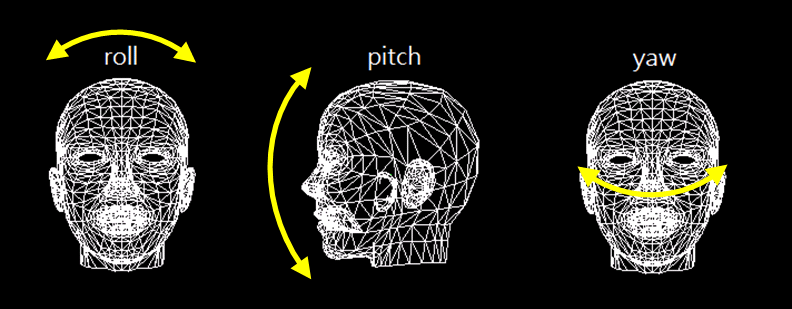
\includegraphics[width=1.0\linewidth]{./fig1.png}
\caption{The threes degree of freedom of head poses: roll, pitch, yaw.}
\label{fig:1}       % Give a unique label
\end{figure}
State-of-the-art methods of head pose estimation can roughly be divided into several categories according to the type of required data (i.e., color image or depth map). The early researches focused on the estimation in color images \cite{Ref15}. The color image-based algorithms can be further divided into two types, feature-based \cite{Ref1,Ref8,Ref10,Ref11,Ref18} and appearance-based \cite{Ref2,Ref4,Ref5,Ref6,Ref7,Ref17} methods. However, those methods relying on color image are sensitive to illumination, and the accuracy will be affected in weak/no light environments.

With the development of fast depth map generating systems such as \cite{Ref12}, many works are inspired to use depth data as additional information to improve color-image based algorithms \cite{Ref1,Ref14,Ref20}, and several recent works use depth data as their primary information \cite{Ref3,Ref9,Ref16,Ref19}. Breitenstein et al. \cite{Ref3} proposed a system which can estimate large rotation angles, but GPU-based implement is required to achieve real-time performance.   On the other hand, the state of the art works \cite{Ref16,Ref19} require training procedure before using the system. We believe that a system with low-complexity and training-free is practical for users.

Recently, Microsoft has released a device, Microsoft Xbox Kinect, which can simultaneously capture color images and their depth information at 30 fps (Fig.~\ref{fig:2}). Kinect uses structured infrared rays to estimate the depth information of the scene, but there are still some limitations. First, the acquired depth map is noisy, that is, the estimated depth values are not constant, and there are flickers in the depth map. The measured flickering rate of per pixel in a static object is about 1.4\% in average. The maximum flickering rate even exceeds 30\% on the edges of objects. Therefore, to adopt such a device, we have to address the noisy data. Secondly, there are many holes within the depth map containing no depth information due to occlusions or transparent materials blocking infrared rays from being received by Kinect. Thirdly, Kinect sensor can’t acquire accurate depth information while objects are too close or too far from camera.  1m~6.5m is an appropriate range for precise depth information. To achieve high accuracy and robustness in our system, we have to address these issues.

\begin{figure*}
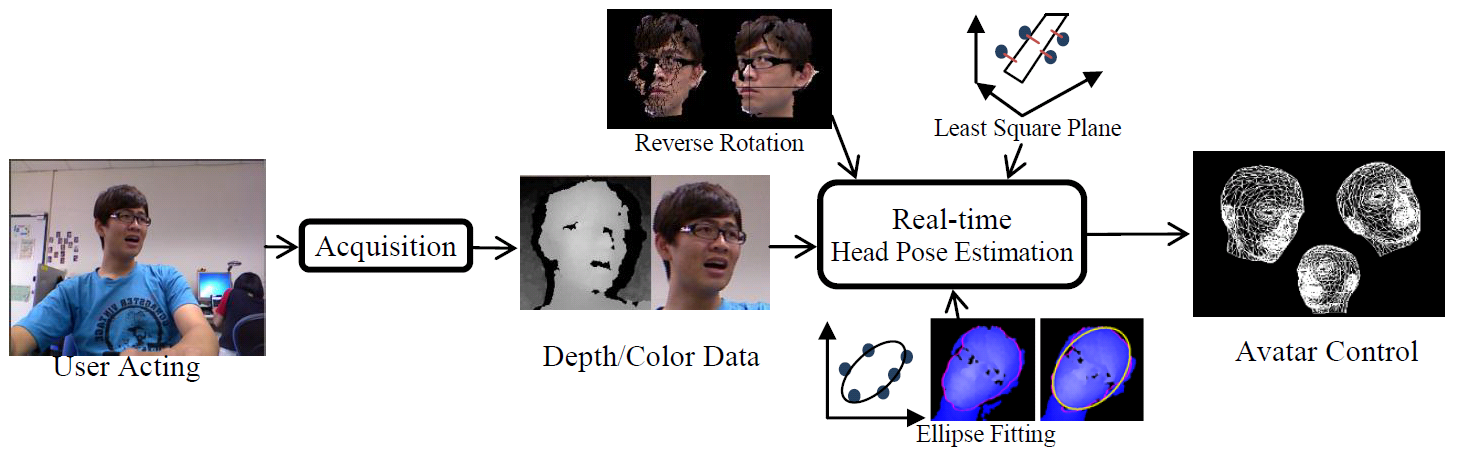
\includegraphics[width=1.0\linewidth]{./fig3.png}
\caption{Visualized overview of the online processing pipeline.}
\label{fig:3}       % Give a unique label
\end{figure*}

\begin{figure}
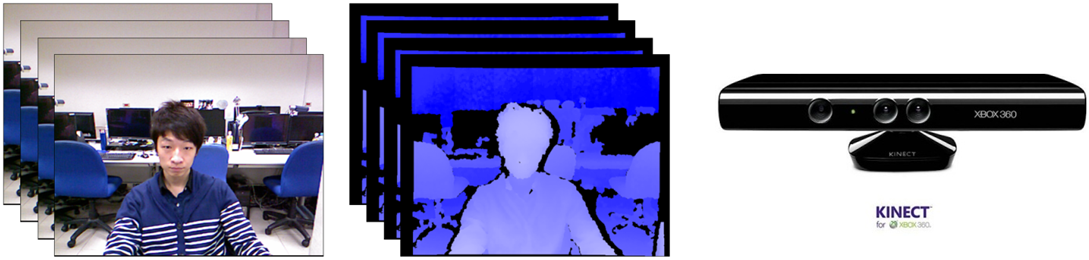
\includegraphics[width=1.0\linewidth]{./fig2.png}
\caption{The color image and corresponding depth map captured by Kinect, both resolution are 640 x 480 at 30 fps.}
\label{fig:2}       % Give a unique label
\end{figure}

\begin{figure}
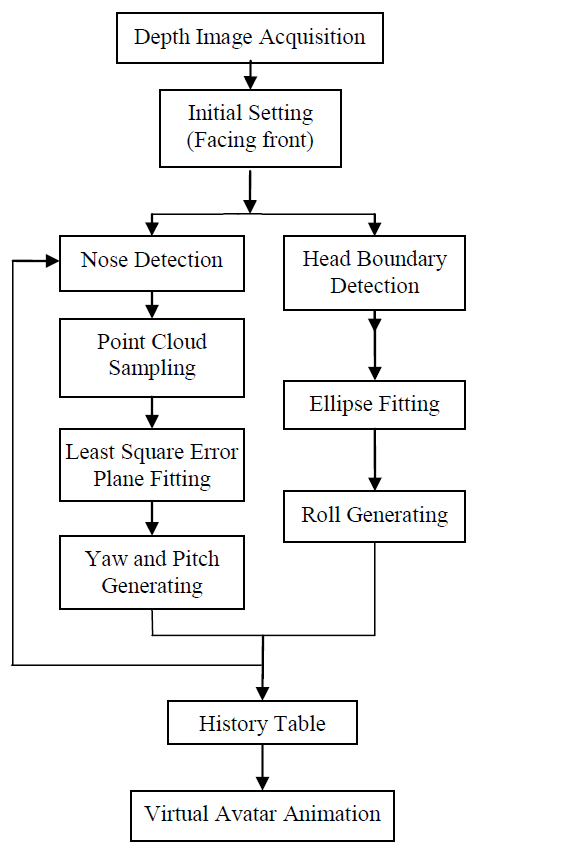
\includegraphics[width=1.0\linewidth]{./fig4.png}
\caption{System flow chart. After data acquisition, the flow can be divided into two parts: Plane fitting for yaw and pitch estimation; Ellipse fitting for roll estimation. The history table keeps tracking the results in order to filter out the outliers and smooth the output parameters.}
\label{fig:4}       % Give a unique label
\end{figure}

In this paper, we propose an approach to estimate the head pose by first locating the nose position. Note that eye positions are hard to detect if without illumination, since the geometry features are not as salient as the nose. Point cloud will  be  sampled  around the nose for generating a least square error plane. Then the normal direction can represent the face orientation. To avoid the impact of lighting conditions, we locate the nose position using only depth information.  Therefore, the only information utilized to estimate head poses is the depth information in our system. The proposed algorithm will be introduced in the following sections.

The rest of this paper is organized as follows. The overview of our system is introduced in Sec.~\ref{sec:2}. The proposed algorithms will be elaborated in Sec.~\ref{sec:3}. Sec.~\ref{sec:4} will show the experimental results. Conclusions and feature work are in Sec.~\ref{sec:5}.


\section{System Overview}
\label{sec:2}
The overview of our system is illustrated in Fig.~\ref{fig:4}, and each square represents a procedure. The initial setting stage requires the subject to face directly to the camera. The processes of head pose estimation are divided into two parts, one for yaw and pitch (left part) angles and the other for roll (right part) angles. In the left part, the nose is located in the depth image using the proposed algorithm. Then several points around the nose are sampled, and we can find a plane to fit the sampled points by the least square method. The plane’s normal vector is used to represent the face orientation. In the right part, the head contour is detected by thresholding the depth values, and then an ellipse is used to fit the head contour. Both the left part and the right part will maintain a history table to preserve the temporal coherence. Finally, the output parameters can be used to control the virtual avatar in real-time.


\section{Implementation}
\label{sec:3}
In general, the head pose can be modeled by six parameters. Three of them are transition parameters respect to x-axis, y-axis and z-axis, and rest of them are rotation parameters - yaw, pitch and roll. Our goal is to estimate these six parameters precisely in real-time while preserving the temporal coherence.

\subsection{Preprocessing}
\label{sec:3.1}
The proposed algorithm uses Microsoft Kinect to capture the depth information. A depth map in VGA resolution is generated with pixel values ranging from 0 to 10,000 millimeters. The depth value can be regarded as the value on z coordinate, and we need to further obtain the values on x and y coordinates. A simple perspective projection model can be used to handle this issue (Fig.~\ref{fig:5}).

\begin{figure}
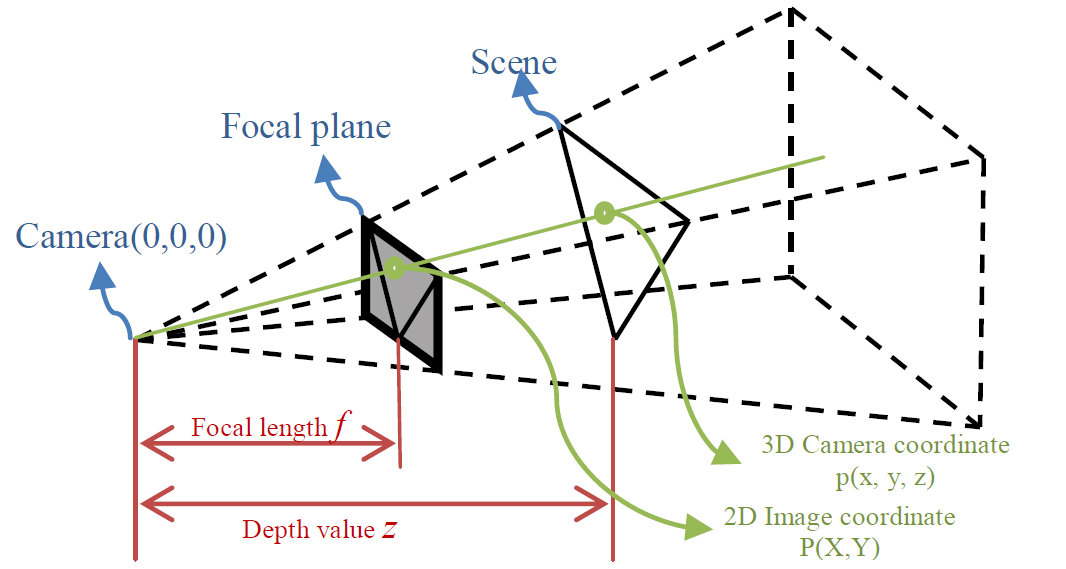
\includegraphics[width=1.0\linewidth]{./fig5.png}
\caption{Perspective projection model which is used in this paper for retrieve the 3D point cloud from Kinect.}
\label{fig:5}       % Give a unique label
\end{figure}

Let the camera as the origin of the 3D world coordinate system and its view direction as the positive z-axis. The focal plane is located at a distance f in front of the camera. A point $p_{3D}(x, y, z)$ on the surface of an object in the 3D scene is projected to a point $P_{2D}(X, Y)$ on the 2D focal plane, where $X=f\cdot x/z, Y=f\cdot y/z$. Since the focal length $f$ of Kinect camera is known already, it can be inferred as the following equation:
\begin{equation}
p=(x,y,z)=(z\cdot \frac{X}{f}, z\cdot \frac{Y}{f}, z)
\end{equation}
Thus the following steps (Sec.~\ref{sec:3.2}, Sec.~\ref{sec:3.3}) can be applied on the 3D point cloud.

\subsection{Transition Estimation}
\label{sec:3.2}
By calculating the center position of the point cloud (See Eq.2), we can easily estimate transition parameters.
\begin{equation}
(t_{x},t_{y},t_{z})=\frac{\sum_{i=1}^n{(x_{i},y_{i},z_{i})}}{N}
\end{equation}

\subsection{Rotation Estimation}
\label{sec:3.3}
We propose a novel algorithm for rotation estimation. The estimation can be divided into two parts: Ellipse fitting for roll angle; Least square error plane fitting for yaw and pitch angles. We use two steps in the fitting procedure. The first step is 2D ellipse fitting which is easier and faster. Although 3D fitting is also possible, the computation complexity is obviously higher and will reduce the performance.  The second step is 3D fitting around the nose area for detecting the “surface normal” of a face. This can be done efficiently since  the fitting is applied to a much smaller area.

\paragraph{Roll Angle Estimation:}
Since the roll angle is decided by fitting the head to an ellipse, the first step is to locate the contour of the head. A depth threshold value is used to filter the background pixels and the leftmost and the rightmost pixels in each row are regarded as the contour (See Fig.~\ref{fig:6}(a)). However, since the captured depth information through Kinect is quite noisy, the detected contour will vary with the time and cause the temporal incoherence problems. For example, the estimated roll angle is not stable, and the virtual avatar will be trembling all the time even there is no head motions. Therefore, we add a smoothness term to handle this issue. The smoothing process adjusts the coordinate of every head contour pixel by an “averaging filter” which is equal to a low-pass filter (Fig.~\ref{fig:6}(b)), using Eq.3 where $(x_{i},y_{i})$ indicates the i-th contour pixel, l means the length of averaging window, which is a constant.

\begin{figure}
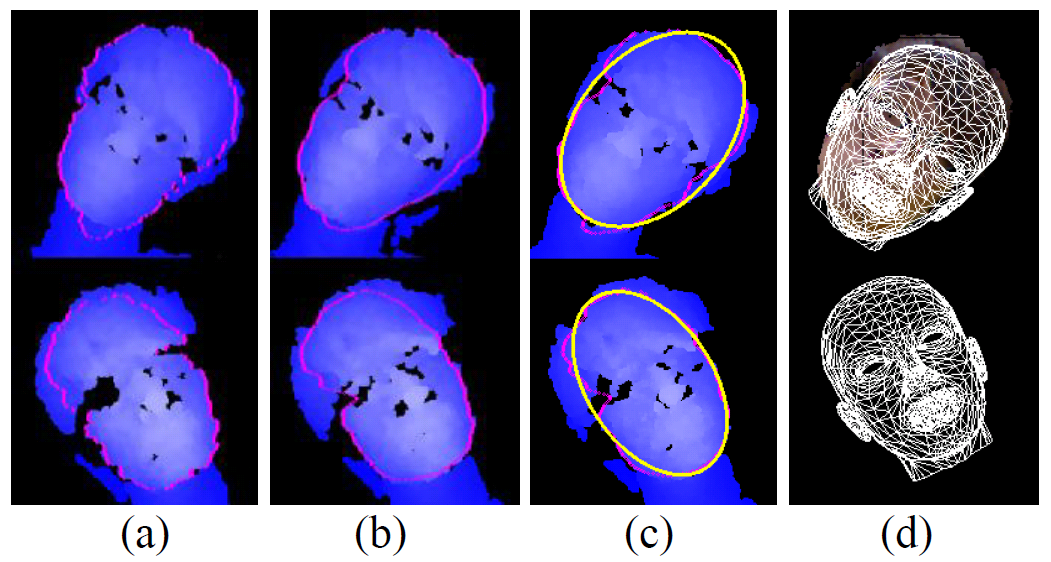
\includegraphics[width=1.0\linewidth]{./fig6.png}
\caption{Detect the boundary of user’s head (a), and smooth the boundary by averaging neighboring points (b). Fit an ellipse that best matches the smoothed head boundary(c), and apply the angle of the result ellipse to the virtual avatar.}
\label{fig:6}       % Give a unique label
\end{figure}

\begin{equation}
(x_{i},y_{i})=\frac{\sum_{k=i-l+1}^{i+l}{(x_{k},y_{k})}}{2\cdot l}
\end{equation}
After the smoothing process, an ellipse is fitted to these contour points by least square error method (See Fig.~\ref{fig:6}(c)). Then we take the rotation angle of the fitted ellipse as the estimated roll angle. Fig.~\ref{fig:6}(d) shows the result.

\paragraph{Pitch and Yaw Angles Estimation}
To estimate yaw and pitch angles, a basic idea is that our faces can be roughly considered as a plane. The normal vector of this plane can represent the orientation of the actor’s face. Our goal is to reconstruct this plane. To achieve this goal, the least square error method is applied to fit a plane to the 3D point cloud. However, Kinect doesn’t provide the information that which of the 3D points belongs to the actor’s face and which doesn’t. Therefore, a face detection process must be applied first. In our work, we achieve this goal by tracking the user’s nose. Fig.~\ref{fig:7} shows the pipeline of this step.

\begin{figure}
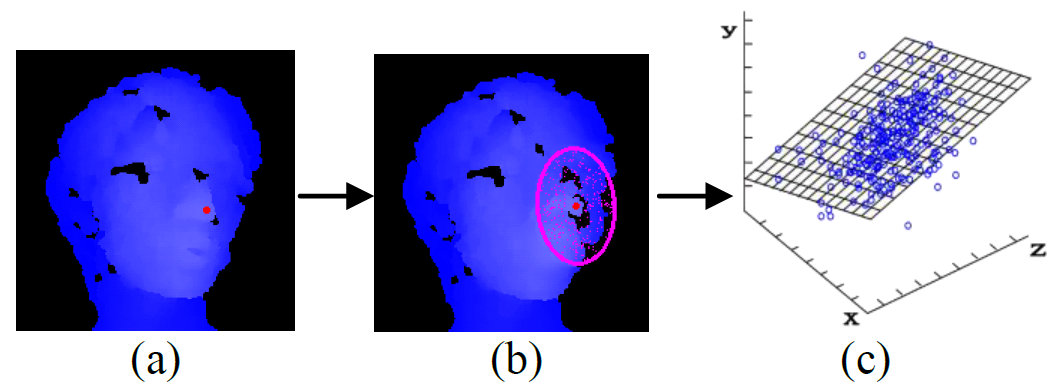
\includegraphics[width=1.0\linewidth]{./fig7.png}
\caption{Detect and track user’s nose (a) and sample several points from the nose’s neighboring area (b) and apply least square error algorithm to fit a plane to the sample points(c).}
\label{fig:7}       % Give a unique label
\end{figure}

It is observed from experiments that human’s nose is the nearest part to the camera at most of the time, except when the user turns his head with extreme large angles. Therefore, we can locate the initial position of nose by finding the shallowest depth value among the point cloud. This assumption remains feasible in a limited range of rotation angles (See Fig.~\ref{fig:8}(a)). However, in some specific conditions, it might appear that other parts on our face keep a shallower value than our nose. For example, glasses or cheek will be the shallowest point when yaw angle surpasses about 20 degrees, and chin and fringe will be the shallowest point when pitch angle surpasses about 15 degrees (See Fig.~\ref{fig:8}(b)).

\begin{figure}
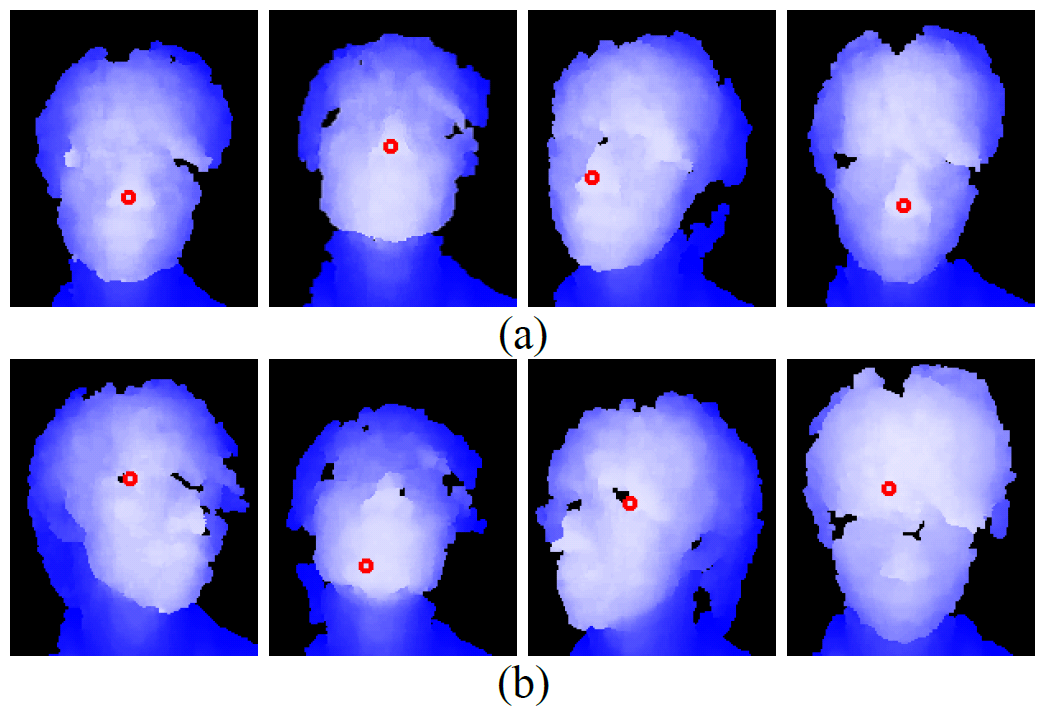
\includegraphics[width=1.0\linewidth]{./fig8.png}
\caption{Nose point has the shallowest depth (to the viewer) value among the point cloud in small rotation range (a), while other parts of the human head will take over the shallowest position (b). Red circle indicates the detected shallowest point (or nearest point to the viewer).}
\label{fig:8}       % Give a unique label
\end{figure}

This problem can be tackled by the following steps. Since a human’s head can only rotate a small range of angles within a short moment such as one thirtieth of a second, we can take advantage of the temporal coherence from previous iterations. The whole point cloud is inversely rotated by the previously estimated yaw and pitch angles so that the currently observed head would turn back to the normal pose.

After this transformation, the new point cloud with new coordinates represent a head that faces straight forward to the camera. Note that the camera stands for the origin of world coordinate. 

\begin{equation}
\begin{bmatrix}
x'\\
y'\\
z'
\end{bmatrix}
=
\begin{bmatrix}
\cos{\theta_{y}}& 0 & -\sin{\theta_{y}}	\\
0 & 1 & 0	\\
\sin{\theta_{y}}& 0 & \cos{\theta_{y}}
\end{bmatrix}
\begin{bmatrix}
1 & 0 & 0	\\
0 & \cos{\theta_{p}} & \sin{\theta_{p}}	\\
0 & -\sin{\theta_{p}} & \cos{\theta_{p}}
\end{bmatrix}
\begin{bmatrix}
x \\
y \\
z
\end{bmatrix}
\end{equation}
Eq.4 Shows the inverse rotation matrix where $\theta_{y}$ and  $\theta_{p}$ represents yaw and pitch angle estimated in the previous iteration:

Even though the adjusted point cloud is not a perfect face 3D model, we can still successfully track the nose by finding the shallowest point as long as the nose can be captured in the depth map. Fig.~\ref{fig:9}(a) illustrates a scenario that user rotates a large angle so other part of his head (green circles in Fig.~\ref{fig:9}(a)) takes over the shallowest position. Since we apply the inverse rotation parameters to make the head face forward (Fig.~\ref{fig:9}(b)), the nose can still keep the shallowest depth value (red circles in Fig.~\ref{fig:9}(a)). Orange arrow shows the inverse rotation direction.

\begin{figure}
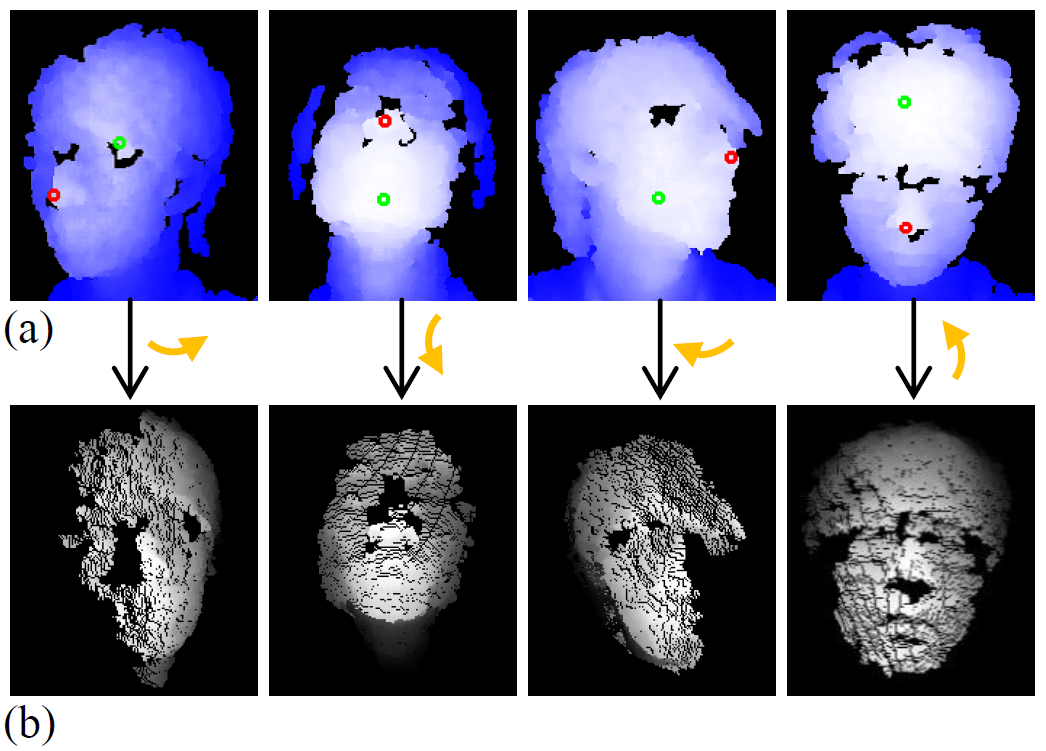
\includegraphics[width=1.0\linewidth]{./fig9.png}
\caption{An inverse rotation transform is applied to the whole point cloud (a) to rotate the head back to the normal pose (b). Green circle indicates the shallowest point while red circle indicates the new shallowest point after inverse rotation.}
\label{fig:9}       % Give a unique label
\end{figure}

As mentioned earlier in this chapter, our faces around the nose area can roughly be considered as a plane. Thus the normal vector of this plane can represent the orientation of the actor’s face. Since our system has detected the user’s nose, we can simply consider the neighboring area of nose to be the face area. In this paper, we sample 300 points from the selected face area (Fig.~\ref{fig:10}), and fit a plane to these sample points by the least square error method. The normal vector of the fitted plane is considered to be the orientation of the face.

\begin{figure}
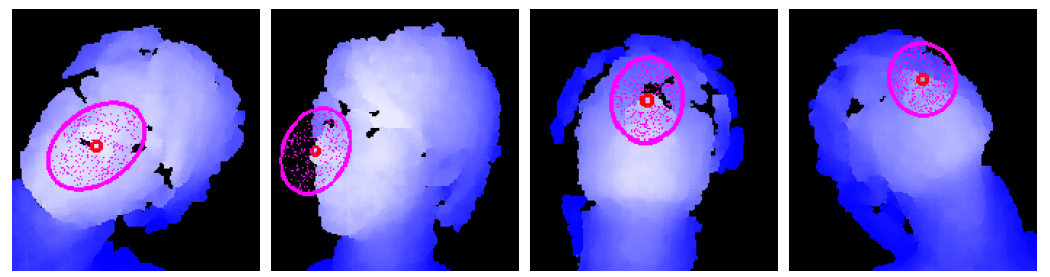
\includegraphics[width=1.0\linewidth]{./fig10.png}
\caption{We sample 300 points from the defined face area, and fit a least square error plane to these sample points. If any sample points happen to be points that have no depth information, ignore them.}
\label{fig:10}       % Give a unique label
\end{figure}

We show an algebraic solution to the least square approximation problem here. Let a plane’s linear equation be $Ax+By+C=z$. Eq.5 indicates that every point sampled from the point cloud is on the plane $Ax+By+C=z$. $(x_{i},y_{i},z_{i})$ is the 3D coordinate of a sample point, and $n$ denotes the number of sample points. 
\begin{small}	%Ax=b
\begin{equation}
\begin{bmatrix}
x_{1} & y_{1} & 1	\\
x_{2} & y_{2} & 1	\\
\vdots & \vdots & \vdots		\\
x_{n} & y_{n} & 1
\end{bmatrix}
\begin{bmatrix}
A	\\
B	\\
C
\end{bmatrix}
=
\begin{bmatrix}
z_{1}	\\
z_{2}	\\
\vdots		\\
z_{n}
\end{bmatrix}
\end{equation}
\end{small}

We can solve this over-determined linear system by Eq.6:
\begin{small}	%ATAx=ATb
\begin{equation}
\begin{bmatrix}
x_{1} & x_{2} & \cdots & x_{n}	\\
y_{1} & y_{2} & \cdots & y_{n}	\\
1 & 1 & \cdots & 1
\end{bmatrix}
\begin{bmatrix}
x_{1} & y_{1} & 1	\\
x_{2} & y_{2} & 1	\\
\vdots & \vdots & \vdots		\\
x_{n} & y_{n} & 1
\end{bmatrix}
\begin{bmatrix}
A	\\
B	\\
C
\end{bmatrix}
=
\begin{bmatrix}
x_{1} & x_{2} & \cdots & x_{n}	\\
y_{1} & y_{2} & \cdots & y_{n}	\\
1 & 1 & \cdots & 1
\end{bmatrix}
\begin{bmatrix}
z_{1}	\\
z_{2}	\\
\vdots		\\
z_{n}
\end{bmatrix}
\end{equation}
\end{small}

After simplification, least square plane coefficients can be obtained by solving Eq.8:
\begin{small}	%(ATA)x=(AT)b
\begin{equation}
\begin{bmatrix}
\sum_{i=1}^{n}{x_{i}^2} 	& \sum_{i=1}^{n}{x_{i}y_{i}}	& \sum_{i=1}^{n}{x_{i}}	\\
\sum_{i=1}^{n}{x_{i}y_{i}} 	& \sum_{i=1}^{n}{y_{i}^2}		& \sum_{i=1}^{n}{y_{i}}	\\
\sum_{i=1}^{n}{x_{i}} 		& \sum_{i=1}^{n}{y_{i}}			& \sum_{i=1}^{n}{1}	
\end{bmatrix}
\begin{bmatrix}
A	\\
B	\\
C
\end{bmatrix}
=
\begin{bmatrix}
\sum_{i=1}^{n}{x_{i}z_{i}}	\\
\sum_{i=1}^{n}{y_{i}z_{i}}	\\
\sum_{i=1}^{n}{z_{i}}
\end{bmatrix}
\end{equation}
\end{small}

We then transform the normal vector $\vec{N}(A,B,-1)$ to yaw and pitch angles. Fig.~\ref{fig:11} illustrates the relation between normal vector $\vec{N}(A,B,-1)$ and pose parameter {yaw,pitch}. $\alpha$ is the angle between $\vec{N}_{yz}$ and negative z-axis and denotes pitch angle, where $\vec{N}_{yz}(0,B,-1)$ is obtained by projecting $\vec{N}(A,B,-1)$ onto y-z plane. On the other hand, $\beta$ is the angle between $\vec{N}_{xz}$ and negative z-axis and denotes yaw angle, where $\vec{N}_{xz}(A,0,-1)$ is obtained by projecting $\vec{N}(A,B,-1)$ onto x-z plane.

\begin{figure}
\centering
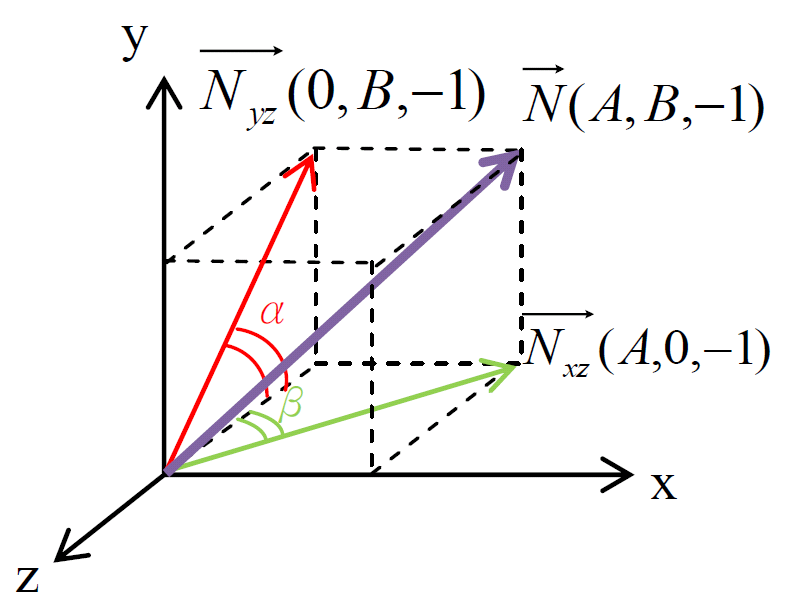
\includegraphics[width=0.7\linewidth]{./fig11.png}
\caption{The relation between normal vector $\vec{N}$ and pose parameter {yaw,pitch}. $\alpha$ denotes pitch angle while $\beta$ denotes yaw angle.}
\label{fig:11}       % Give a unique label
\end{figure}

We apply a simple trigonometric function to the normal vector in order to transform $\vec{N}(A,B,-1)$ to $(\alpha,\beta )$ :
\begin{equation}
\alpha = \arccos{(\frac{1}{\sqrt{A^2+1^2}})},
\beta  = \arccos{(\frac{1}{\sqrt{B^2+1^2}})}
\end{equation}

\subsection{Flickering Problem}
\label{sec:3.4}
Although depth cameras such Kinect can provide depth information in real-time, the accompanying noise in the depth maps will cause the decrease of accuracy in estimation. Therefore, we have to address the problem of data flickering or missing in sequences of depth information. We apply a dynamic temporal filter similar to that of \cite{Ref19} to solve flickering problem. In addition to the smoothness in depth maps, a history table is maintained to record the estimated results in each frame. Therefore, we can ignore impossible transitions of head poses by tracking the table. For instance, 60 degrees of yaw angle comes right after 5 degrees of yaw angle. 
\section{Results}
\label{sec:4}
Fig.~\ref{fig:12} shows the results from three users of which each makes ten arbitrary pose. The first and fourth columns show what pose users make. Note that our system doesn’t take any advantage from these color images so that it still performs well when the there is no lighting in the environment. The second and fifth columns are the depth maps captured by the 3D sensor. The third and sixth columns show visualizations of the results by using the output parameters to control virtual avatars. We implement our system on a PC with Intel CPU Q9500 (2.83 GHz) and NVIDIA 210 graphics display card, and can currently achieve 30 fps.

\begin{figure}
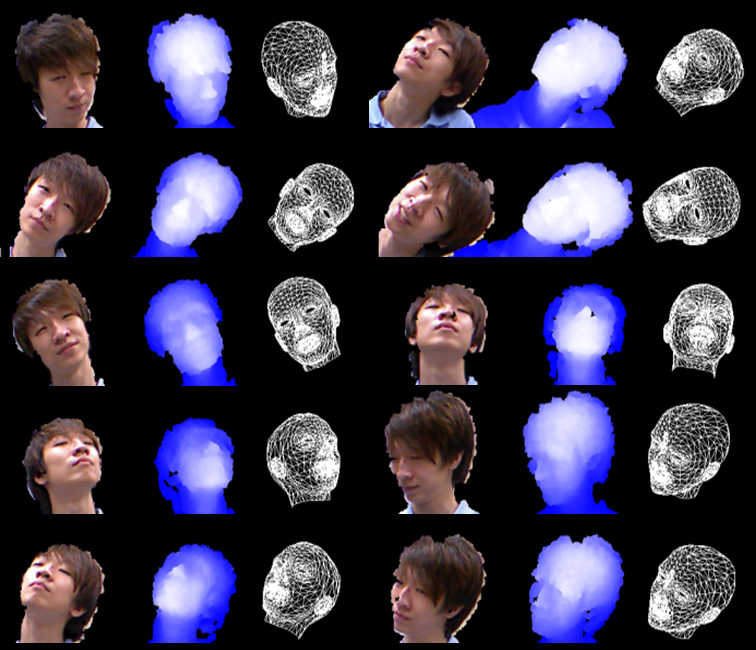
\includegraphics[width=1.0\linewidth]{./fig12a.png}
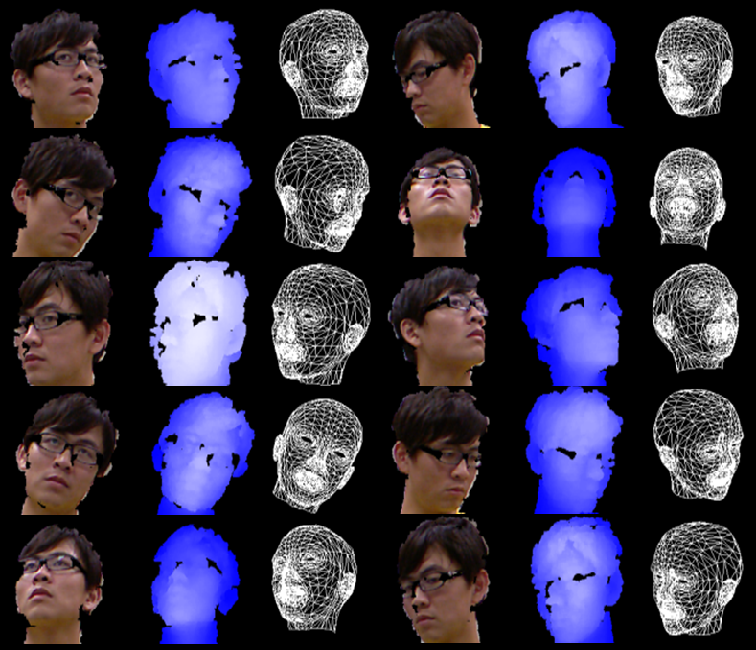
\includegraphics[width=1.0\linewidth]{./fig12b.png}
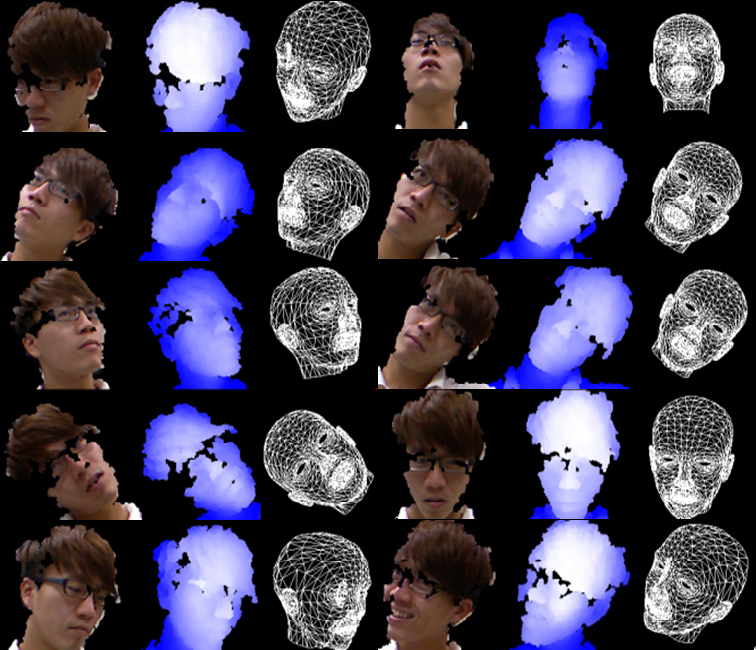
\includegraphics[width=1.0\linewidth]{./fig12c.png}
\caption{The experimental results of three different males for performing head pose, each one has different nose size and hair fringe. The result also shows that wearing eyeglasses will not decrease the accuracy.}
\label{fig:12}       % Give a unique label
\end{figure}

From the results, we observed that the estimated roll angle is quite robust by utilizing the proposed algorithm. In a formal experiment, 14 people were tested. In general, for the maximum working range angles, $\pm 45^{\circ}$ around the initial “front facing” position can be achieved. In our “avatar control” application, this is already useful and enough, although we will try to extend the maximum angles to around $\pm 90^{\circ}$ in the future. Currently, the roll angle can reach already $\pm 70^{\circ}$. However, the estimation may fail for the yaw and pitch angles if we can’t successfully detect the nose which is the key feature used in the proposed algorithm. In this case, manual refocusing is possible. In general case, where no hair fringe or hair blocking, the accuracy is around 100\%, and with hair blocking (especially female faces) the accuracy is 96\%.

It is also observed from the experiments that the hair style may affect the estimation. Long hairs may interfere in the procedure of face boundaries detection and cause the decrease of accuracy in roll angle estimation (as shown in the left-bottom of Fig.~\ref{fig:13}). Fortunately, the estimation in yaw and pitch angles will not be affected by the hair style.

\begin{figure}
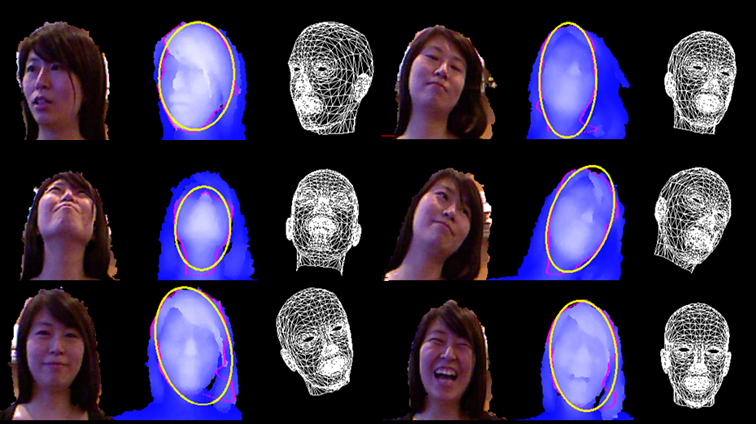
\includegraphics[width=1.0\linewidth]{./fig13.png}
\caption{esults of female users are as accurate as male users in terms of yaw and pitch angles while long hair may affect the boundary detection and further decrease accuracy of roll angle estimation (left-bottom). The right-bottom picture shows that dramatic facial expression doesn’t affect the estimation.}
\label{fig:13}       % Give a unique label
\end{figure}

\section{Conclusion and Future Work}
\label{sec:5}
In this paper, we propose a real-time head pose estimation system that only requires the depth information. There are three key features in our system: 1) The estimation is based on the nose tracking and requires low computation cost. 2) Calibrations, training procedures, and registrations are not required. 3) Cheap and commercially available 3D sensors make our system easy to setup.

In a formal experiment, 14 people were tested. In general, for the maximum working range angles, $\pm 45^{\circ}$ around the initial “front facing” position can be achieved. Currently, the roll angle can reach already $\pm 70^{\circ}$. In general case, where no hair fringe or hair blocking, the accuracy is around 100\%, and with hair blocking (especially female faces) the accuracy is 96\%.


% For tables use
%\begin{table}
% table caption is above the table
%\caption{Please write your table caption here}
%\label{tab:1}       % Give a unique label
% For LaTeX tables use
%\begin{tabular}{lll}
%\hline\noalign{\smallskip}
%first & second & third  \\
%\noalign{\smallskip}\hline\noalign{\smallskip}
%number & number & number \\
%number & number & number \\
%\noalign{\smallskip}\hline
%\end{tabular}
%\end{table}


%\begin{acknowledgements}
%If you'd like to thank anyone, place your comments here
%and remove the percent signs.
%\end{acknowledgements}

% BibTeX users please use one of
%\bibliographystyle{spbasic}      % basic style, author-year citations
%\bibliographystyle{spmpsci}      % mathematics and physical sciences
%\bibliographystyle{spphys}       % APS-like style for physics
%\bibliography{}   % name your BibTeX data base

% Non-BibTeX users please use
\begin{thebibliography}{}
%
% and use \bibitem to create references. Consult the Instructions
% for authors for reference list style.
%


%\bibitem{RefJ}
% Format for Journal Reference
%Author, Article title, Journal, Volume, page numbers (year)

\bibitem{Ref1}
R. Yang, and Z. Zhang, Model-based head pose tracking with stereovision, Proceedings of IEEE International Conference on Automatic Face and Gesture Recognition, pp. 255-260, 2002.

\bibitem{Ref2}
L.-P. Morency, P. Sundberg, and T. Darrell, “Pose estimation using 3d view-based eigenspaces, ” Proceedings of the IEEE International Workshop on Analysis and Modeling of Faces and Gestures, pp. 45-52, 2003.

\bibitem{Ref3}
M. D. Breitenstein, D. Kuettel, T. Weise, L. Van Gool, and H. Pfister, “Real-time face pose estimation from single range images,” IEEE Conference on Computer Vision and Pattern Recognition, pp. 1-8, 2008.

\bibitem{Ref4}
V. N. Balasubramanian, J. Ye, and S. Panchanathan, “Biased manifold embedding: A framework for person-independent head pose estimation,” IEEE Conference on Computer Vision and Pattern Recognition, pp. 1-7,  2007.

\bibitem{Ref5}
M. Osadchy, M. L. Miller, and Y. LeCun, “Synergistic face detection and pose estimation with energy-based models,” Journal of Machine Learning Research, Vol. 8, pp.1197 – 1215, 2007

\bibitem{Ref6}
M. Storer, M. Urschler, and H. Bischof, “3d-mam: 3d morphable appearance model for efficient fine head pose estimation from still images,” Proceedings of IEEE International Conference on Computer Vision,Workshop on Subspace Methods, pp. 192 – 199, 2009.

\bibitem{Ref7}
M. Jones, and P. Viola, “Fast multi-view face detection,” Technical Report TR2003-096, Mitsubishi Electric Research Laboratories, 2003.

\bibitem{Ref8}
T. Vatahska, M. Bennewitz, and S. Behnke, “Feature-based head pose estimation from images,” Proceedings of IEEE-RAS International Conference on Humanoid Robots, pp. 330 - 335, 2007.

\bibitem{Ref9}
S. Malassiotis, and M. G. Strintzis, “Robust real-time 3d head pose estimation from range data,” Pattern Recognition, vol.38, no. 8, pp.1153 – 1165, 2005.

\bibitem{Ref10}
Y. Matsumoto and A. Zelinsky, “An algorithm for real-time stereo vision implementation of head pose and gaze direction measurement,” Proceedings of IEEE International Conference on  Automatic Face and Gesture Recognition, pp. 499 - 504, 2000.

\bibitem{Ref11}
J. Yao, and W. K. Cham, “Efficient Model-Based Linear Head Motion Recovery from Movies,” Proceedings of IEEE Computer Society Conference on Computer Vision and Pattern Recognition, Vol. 2, pp. II-414-II-421,  2004.

\bibitem{Ref12}
T. Weise, B. Leibe, and L. Van Gool, “Fast 3D Scanning with Automatic Motion Compensation,” Proceedings of IEEE Computer Society Conference on Computer Vision and Pattern Recognition, pp. 1-8, 2007.

\bibitem{Ref13}
Q. Cai, D. Gallup, C. Zhang, and Z. Zhang, “3D Deformable Face Tracking with A Commodity Depth camera,” European Conference on Computer Vision, pp. 229-242, 2010.

\bibitem{Ref14}
L.-P. Morency, P. Sundberg, and T. Darrell, “Pose Estimation Using 3D View-Based Eigenspaces,” Proceedings of the IEEE International Workshop on Analysis and Modeling of Faces and Gestures, pp. 45-52, 2003.

\bibitem{Ref15}
E. Murphy-Chutorian, and M. Trivedi, “Head Pose Estimation in Computer Vision: A Survey,” IEEE Transactions Pattern Analysis and Machine Intelligence, Vol. 31, No. 4, pp. 607–626,  2009.

\bibitem{Ref16}
G. Fanelli, J. Gall, and L. V. Gool, “Real Time Head Pose Estimation with Random Regression Forests,” Proceedings of IEEE Computer Society Conference on Computer Vision and Pattern Recognition, 2011.

\bibitem{Ref17}
L. Chen, L. Zhang, Y. Hu, M. Li, and H. Zhang, “Head Pose Estimation Using Fisher Manifold Learning,” Proceedings of the IEEE International Workshop on Analysis and Modeling of Faces and Gestures, pp. 203-207, 2003.
 
\bibitem{Ref18}
J. Whitehill, and J. R. Movellan, “A Discriminative Approach to Frame-by-Frame Head Pose Tracking,” Proceedings of the IEEE International Conference on Analysis and Modeling of Faces and Gestures, pp. 1-7, 2008.

\bibitem{Ref19}
T. Weise, S. Bouaziz, H. Li, and M. Pauly, “Real time Performance-Based Facial Animation,” ACM Transactions on Graphics, Proceedings of the 38th ACM SIGGRAPH Conference and Exhibition, 2011.

\bibitem{Ref20}
E. Seemann, K. Nickel, and R. Stiefelhagen, “Head Pose Estimation Using Stereo Vision for Human-Robot Interaction,” Proceedings of the IEEE International Conference on Analysis and Modeling of Faces and Gestures, pp. 626-631, 2004.


% Format for books

%\bibitem{RefB}
%Author, Book title, page numbers. Publisher, place (year)
% etc

\end{thebibliography}

\end{document}
% end of file template.tex

